\section{Librería}
\label{qlib}

La librería creada por este trabajo recibe el nombre de QLib. El objetivo de la creación de la librería es brindar una base de código que permita
la creación o modificación de herramientas para la enseñanza del lenguaje en el ecosistema de javascript, brindando así la posibilidad de ser
utilizada en navegadores web.
Además la existencia de una librería así, permite la creación de interfaces de usuario que extiendan a la entregada en este trabajo.

La misma esta compuesta por tres capas principales: Parser, Translator y Computer. Las funcionalidades que ofrece son:

\begin{itemize}
  \item Implementación del lenguaje Q: todas las instrucciones de Q, modos de direccionamiento, registros, flags, PC, SP, IR, MAR, MBR, etiquetas, pila están implementadas.
  \item Manejo de etiquetas: se proveen mecanismos para definir etiquetas, asociarlas a una dirección y utilizarlas en el ensamblado de programas.
  \item Manejo del ensamblado: métodos para pasar de un programa Q a la representación binaria de las instrucciones y viceversa.
  \item Ejecución completa, paso a paso y paso a paso detallada.
  \item Parseo del código Q.
  \item Capa de traducción entre el parseo y las instrucciones de la librería \referencia{subsec:translator}. 
  \item Opciones de configuración de la librería: modificar la cantidad de registros, valores por defecto de celdas y registros, modos de direccionamiento e instrucciones habilitadas en la ejecución.
  \item Exposición de valores del estado a lo largo de la ejecución.
  \item Exposición de acciones realizadas a lo largo de la ejecución.
\end{itemize}

Está diseñada utilizando el paradigma de programación orientada a objetos el cual define la existencia de clases y sus interacciones. 

\subsection{Parser}

El parser es la unidad encargada del analisis sintáctico para determinar si el programa es correcto de acuerdo a la gramática del lenguaje Q. 
Recibe como entrada una cadena de texto y devolverá objetos javascript en caso de ser la entrada sintacticamente válida o un error en caso 
contrario. Dicha salida será la entrada del Translator \referencia{subsec:translator}.

Para la definición de la gramática y su análsis sintáctico se utilizó la librería nearley.js, la cual provee una sintaxis para la definición de 
gramáticas basada en \textit{Extended Backus-Naur Form}. Los detalles de EBNF escapan al desarrollo de este trabajo por lo que es suficiente con 
pensar que este funciona como un metalenguaje, es decir, un lenguaje que permite la construcción de otros lenguajes. 

Para utilizar nearley.js se genera un archivo de gramática con la extensión .ne, donde se define la idea de instrucción, operando, tipos de 
instrucción y etiquetas. Luego, dicho archivo se compila a javascript utilizando la librería y esto permite el uso de la gramática en navegadores.

Una vez que la gramática está compilada, se utilizará la clase Parser provista por la librería para ingresar las instrucciones en forma de texto. 
Si son sintacticamente correctas, se devolverá un objeto preparado para traducirse a las instrucciones del lenguaje Q.

Este diseño que separa la etapa de parseo de la etapa de traducción a las clases del lenguaje permite la utilización de un parser distinto, siempre y cuando
su salida respete el formato esperado por el Translator.

\begin{figure}[H]
  \centering
  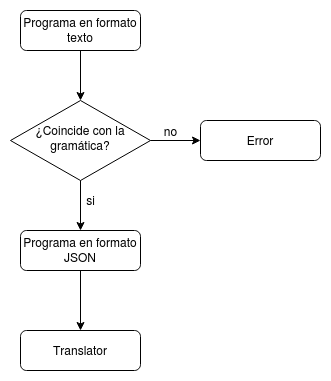
\includegraphics[width=7cm]{figuras/parser.png}
  \caption{Proceso de parseo del código.}
\end{figure}


\subsection{Translator}
\label{subsec:translator}
Como uno de los objetivos de QLib es permitir su utilización con distintos parsers, se provee una capa que actúe de interfaz entre los resultados 
brindados por el parser y las rutinas que utilizará la clase Computer para ejecutar el programa. 

En él se definen un conjunto de reglas que determinan cómo mapear las posibles entradas de formato JSON a instrucciones soportadas por QLib. Estas reglas 
se dividen en 3 grupos: \textit{reglas para instrucciones}, para \textit{tipos de instrucciones} y \textit{para operandos}.

\begin{figure}[H]
  \centering
  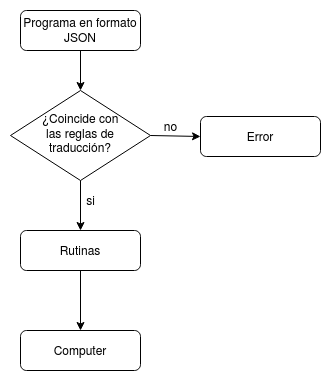
\includegraphics[width=7cm]{figuras/translator.png}
  \caption{Proceso de traducción del código.}
\end{figure}

Cuando se quiere traducir un programa, se realiza el siguiente proceso línea por línea:

En base a la línea que se está traduciendo, se busca una instrucción que coincida con el nombre de la misma en las \textit{reglas para 
instrucciones}. Una vez encontrada la instrucción, se busca el tipo de la instrucción en las \textit{reglas de tipos}. El tipo de la instrucción sirve para determinar
cómo se traducirán los operandos. Luego se obtienen los operandos de acuerdo al tipo de instrucción y el nombre del operando en las \textit{reglas para operandos}, 
obteniendo así, una instancia de operando de QLib. Con estas búsquedas realizadas se puede instanciar la instrucción de QLib y así armar las rutinas.